\section{Architectural Design}

The purpose of this section is to present and analyze the architecture of the software to be system in a top-down manner. We first introduced the overall architecture and then provided a diagram of the system’s components, focusing on the tournaments and battles sub-components. Next, we used an ER diagram to describe the system’s logical data and presented the system’s deployment view, including the layers and tiers involved. We also used sequence diagrams to depict important runtime views and class diagrams to analyze the component interfaces. Finally, we discussed the architectural design choices and the reasons behind them.

\subsection{Overview}
The figure shown below represents a high-level description of the components which make up the System.
It is a distributed system with a 4-tier architecture: presentation, web server, application server and database. In this document, the presentation layer and the Client will be referred to as the Frontend, while the Application Layer and the Data Layer will be referred to as the Backend.
\\
\begin{figure}[h]
    \center
    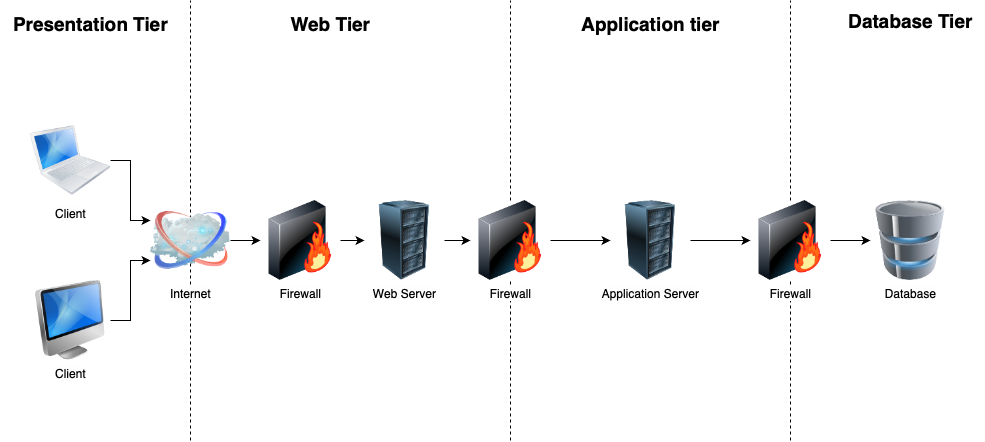
\includegraphics[width=1\linewidth]{src/High level system architecture.png}
    \caption{High level system architecture}
    \label{fig:High level system architecture}
\end{figure}
\\
The presentation tier is the client side, where users interact with the system through a web browser. A single page application will be developed both for educators and students to use the system. The reason behind this choice is the ease of interaction without the need for frequent page reloading, providing a better user experience.\\
The web server is responsible for communication between the Frontend and the Backend. It handles HTTP requests, routing them to the appropriate components. It supports secure communication with clients through HTTPS, and load balancing ensures optimal performance during periods of high traffic.\\
The application tier is the logic core of our system. It processes data received from the presentation tier, performs business logic operations, and communicates with the database. It tier ensures data integrity, security, and authentication, with role-based access controls. It interfaces with external services or APIs as needed. \\
Finally, the data tier is responsible for storing, reading and updating all information necessary for the system. We use a relational database that offers high scalability potential for structured data.
It interfaces with the application tier, granting data access and manipulation while respecting security protocols.\\
The client web-server and web-server application-server communication use HTTP, while app-server DBMS communication relies on APIs. The app-servers are designed to be stateless according to REST standards. The system also includes firewalls to enhance security.\\

\vspace{1cm}

\subsection{Component view}
In this section we offer a more detailed view of the S2B. We will focus on the components and their interactions, along with the interfaces. To meet performance and availability criteria, most of said components will be duplicated or replicated.
\begin{figure}[ht]
    \centering
    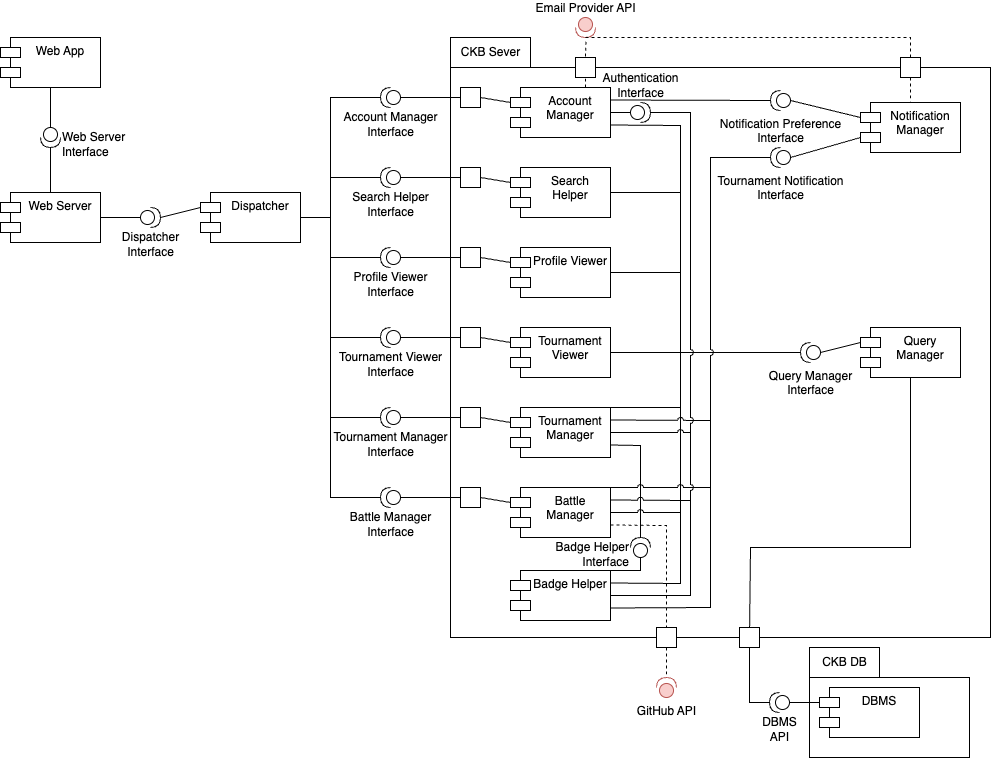
\includegraphics[width=1\linewidth]{src/Component Diagram of the CKB System.png}
    \caption{Component Diagram of the CKB System}
    \label{fig:Component Diagram of the CKB System}
\end{figure}
\\
\newpage

\begin{itemize}
    \item \textbf{Web server}\\
    The web server is designed to handle HTTP requests from the client, redirecting them to the appropriate components. It uses client-side rendering. As the user interacts with the page, further requests may be automatically made and the page will be updated dynamically without requiring a full page reload.\\
    \item \textbf{CKB server}\\
    The CKB server is responsible for the business logic and provide the full functionality to users. Since most of the functionalities offered are shared between educators and students, there will not be a different server for each user category. It is further composed of different components.\\
    \begin{itemize}
        \item \textbf{CKB’s Account Manager}\\
        This component handles all the account operations related to the users and offers an interface to authenticate the requests. It offers functionality to create new account, logging in, setting preferences and verify the authentication of the user at any time. To create a new account, It interacts with the external email provider API to make the user receive a code to verify the identity.\\
        \item \textbf{Search helper}\\
        This component enables the search functionality, letting users and non-users search for a specific user or a specific tournament. It also allows filtering based on date posted, number of awards, ongoing/finished, number of participants and much more (tournaments).\\
        \item \textbf{Profile viewer}\\
        This component allows viewing profiles of users subscribed to CKB, both educators and students. Anyone can see profiles, even unsubscribed users. Within the profile page, there may be tournaments the user took part in (as a student or as an educator) and clicking them will redirect that tournament page.\\
        \item \textbf{Tournament viewer}\\
        This component allows viewing tournaments, along with the battle pages in the scope of It. Anyone can see tournaments, even unsubscribed users. You can find all the information related to that tournament, as well as the battles, including teams, final rank for each battle and much more.\\
        \item \textbf{Tournament manager}\\
        This component allows managing and creating tournaments for educators and subscribing to them for students. The creator can grant other educators permission to create battles. For ongoing tournaments, allowed educators can create new battle clicking the right button. Such functionality is provided through the next component.\\
        \item \textbf{Battle manager}\\
        This component allows managing and creating battles for educators and joining them for students. It also manages the team functionality, allowing students to team up for each battle as well as the scores for each team (including manual evaluation) \\
        \item \textbf{Badge helper}\\
        This component enables the gamification aspects of CKB. It allows educators to create badges and define new rules as well as new variables associated with them. Badges are then linked to the profile of users achieving them, making them visible to anyone.\\
        \item \textbf{CKB Notification Service}\\
        This component enables the CKB notifications. Users will receive notifications about important events, like new tournaments created, tournament to which the user is subscribed closes and more.
        \newline
        \newline
        \textbf{External APIs}\\
        \item \textbf{GitHub API}\\
        This API enables the GitHub integration: new repositories automatically created (e.g. when a new battle begins) and sources automatically downloaded (e.g. when a user pushes new code to the main branch of his repository)\\
        \item \textbf{Email provider API}
        This service is used for authentication during registration.
    \end{itemize}
    \vspace{1cm}
    \item \textbf{Query Manager}
    \\This component is responsible for communicating with the Database Management System. It follows the adapter pattern, allowing  easier communication between other components and the DBMS.
\end{itemize}

\newpage

\subsection{Deployment view}
This chapter describes the deployment of the system.
\begin{figure}[ht]
    \centering
    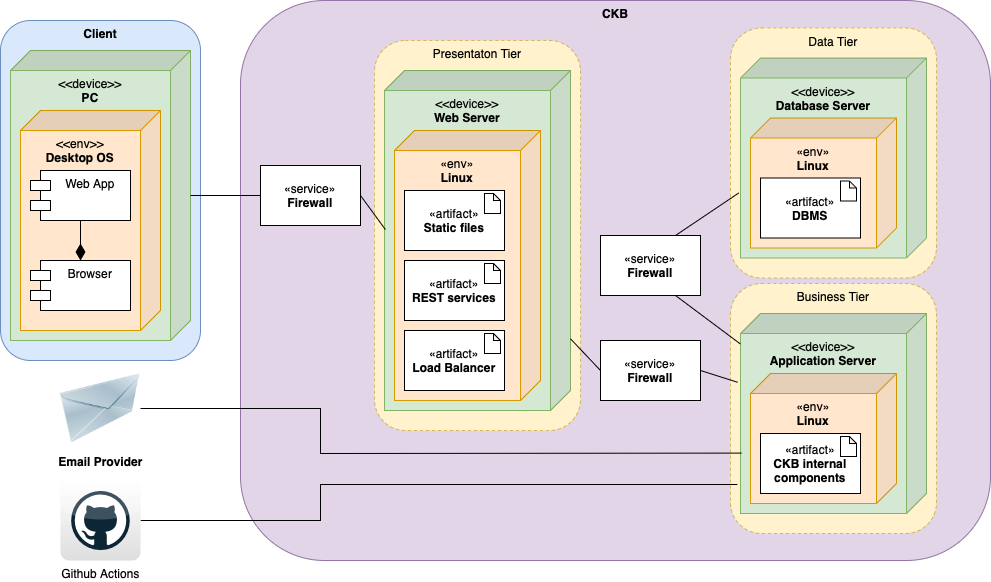
\includegraphics[width=1\linewidth]{src/Deployment View of the system.png}
    \caption{Deployment View of the system}
    \label{fig:Deployment View of the system}
\end{figure}
\\
\begin{itemize}
    \item \textbf{Web-server}\\
    The web-server will be the entry point for the SPA. It forwards the requests to the application-server. A modern device with access to a web browser is required to interface with the web-server. 
    \item \textbf{Load Balancer}\\
    This device is responsible for load balancing, which means, distributing incoming network traffic and requests across multiple servers. Its primary purpose is to optimise resource utilization, enhance reliability while ensuring high availability.
    \item \textbf{Firewall}\\
    Firewalls are used to filter connections to the application and data layers of a system. They are located between the internet and the system intranet. They offer additional security blocking or allowing traffic based on predetermined rules.
\end{itemize}

\newpage

\subsection{Runtime View}
This section illustrates the interactions between actors, subsystems and interfaces of the system showing the specific method called.
\subsubsection{Runtime View Preconditions}{
    \begin{itemize}
        \item \textbf{Web Server views}\\
        The calls to the web server for retrieve the views of each page are implied and not explicitly shown in the runtime views below. 
        Notice that the Web server will act as a proxy when it has already the requested page.
        \item \textbf{Token Validation}\\
        Users can only search and view details of  tournaments and profiles without first being authenticated and authorized. All other actions that a user (both students and educators) can perform are dependent on the validation of a token. The token is passed in the API request and the process of verifying it is shown in the sequence diagram below.
        \begin{figure}[h]
            \centering
            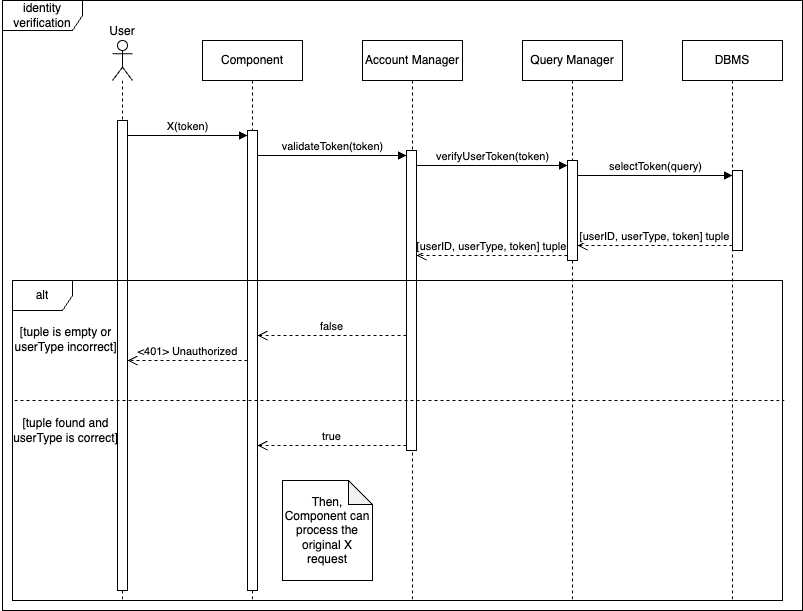
\includegraphics[width=1\linewidth]{src/Token validation.png}
            \caption{Token validation}
            \label{fig:Token validation}
        \end{figure}
    \end{itemize}
}
\newpage
\begin{itemize}
    \item \textbf{Log in}\\
    The user must login in order to join or create tournaments and battles. The user enters the credentials (email and password) and, if they are valid, he will be authenticated, 
    otherwise, an error will be displayed.
    \begin{figure}[h]
        \centering
        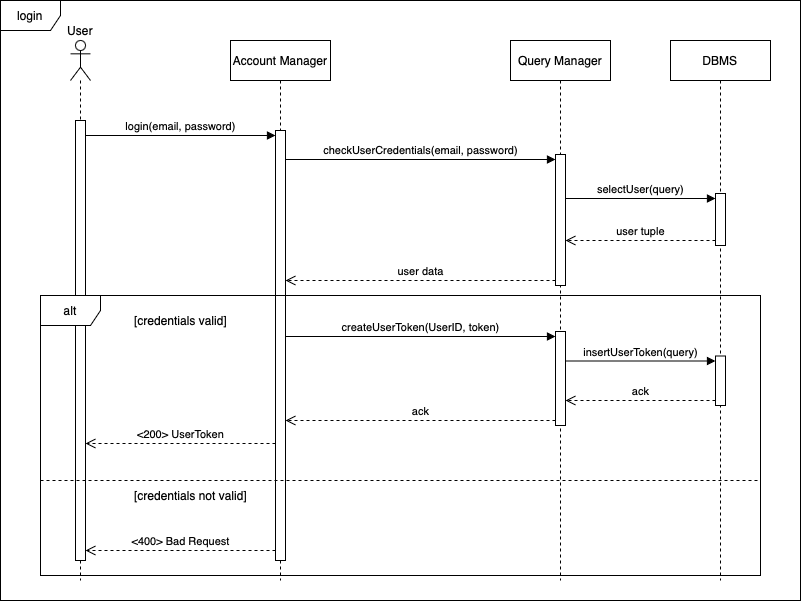
\includegraphics[width=1\linewidth]{src/Login.png}
        \caption{Login}
        \label{fig:Login}
    \end{figure}
    \newpage
    \item \textbf{Registration}\\
    This is the process a new user must follow to create a new account. First, they enter their desired credentials. Then, the system checks if the email provided already belongs to 
    another user. If It does not, a new account is created and a confirmation email is sent. Otherwise, an error will be displayed.
    \begin{figure}[h]
        \centering
        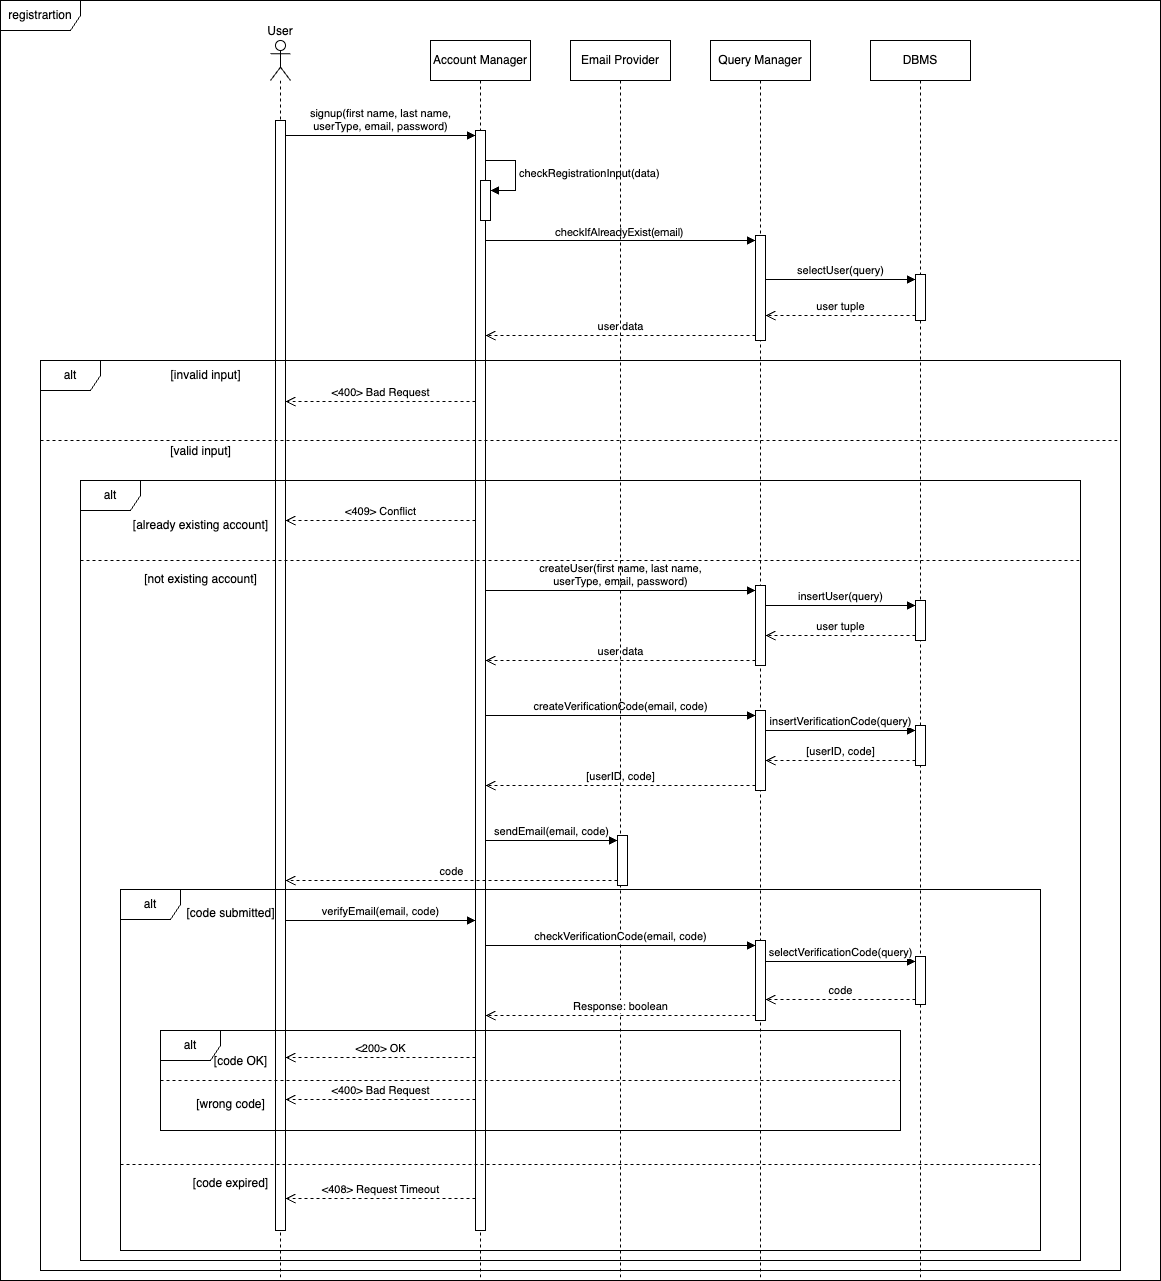
\includegraphics[width=1\linewidth]{src/Registration.png}
        \caption{Registration}
        \label{fig:Registration}
    \end{figure}
    \newpage
    \item \textbf{See tournament}\\
    Users can search for tournaments by name and applying filters. Requests will be handled by the search helper. After a user clicks on their desired tournament, the right page 
    will be shown thanks to the tournament viewer. 
    \begin{figure}[h]
        \centering
        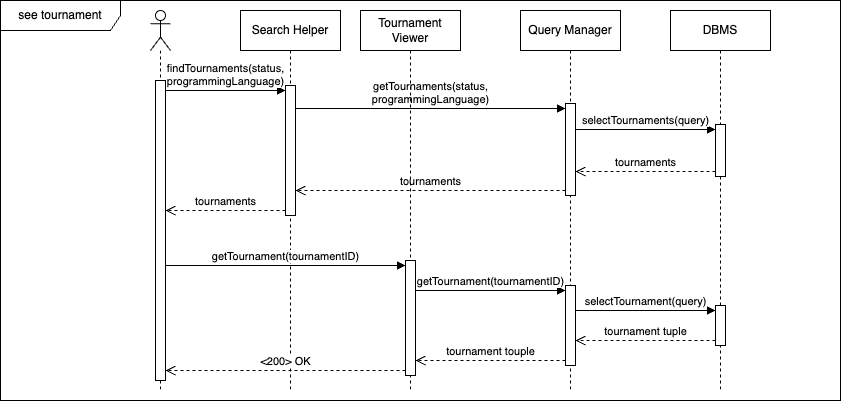
\includegraphics[width=1\linewidth]{src/See tournament.png}
        \caption{See tournament}
        \label{fig:See tournament}
    \end{figure}
    \vspace{1cm}
    \item \textbf{See profile}\\
    Users can search for profiles by name and applying filters. Requests will be handled by the search helper. After a user clicks on their desired profile, the right page 
    will be shown thanks to the profile viewer.
    \begin{figure}[h]
        \centering
        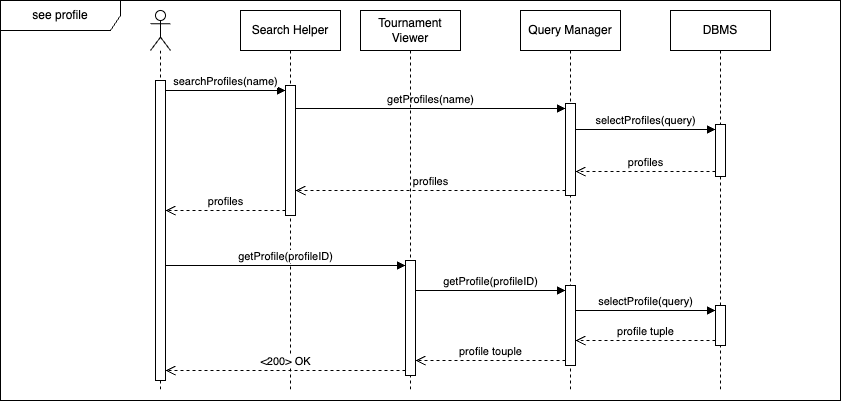
\includegraphics[width=1\linewidth]{src/See profile.png}
        \caption{See profile}
        \label{fig:See profile}
    \end{figure}
    \newpage
    \item \textbf{Manage account}\\
    Requests are handled by CKB's account manager. Users can update their desired preferences.
    \begin{figure}[h]
        \centering
        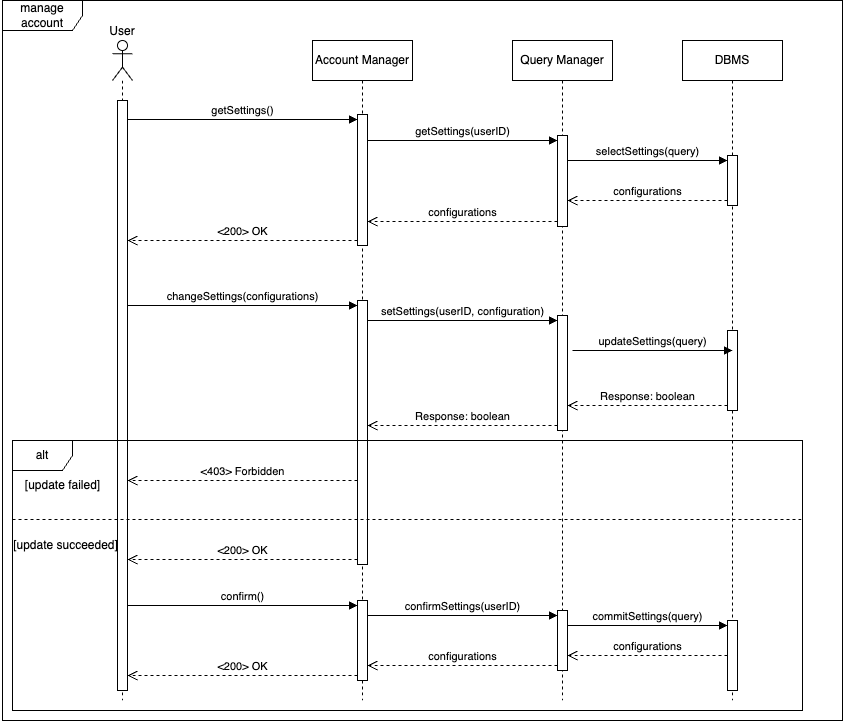
\includegraphics[width=1\linewidth]{src/Manage account.png}
        \caption{Manage account}
        \label{fig:Manage account}
    \end{figure}
    \newpage
    \item \textbf{Join tournament}\\
    The user navigates to the tournament they are interested in thanks to the tournament viewer as shown before. If the user is logged in as a student, a 'join tournament' button is displayed that the user can click. The request is handled by the tournament manager. If the request is valid, the user successfully joins the tournament. Internal databases are updated accordingly.
    \begin{figure}[h]
        \centering
        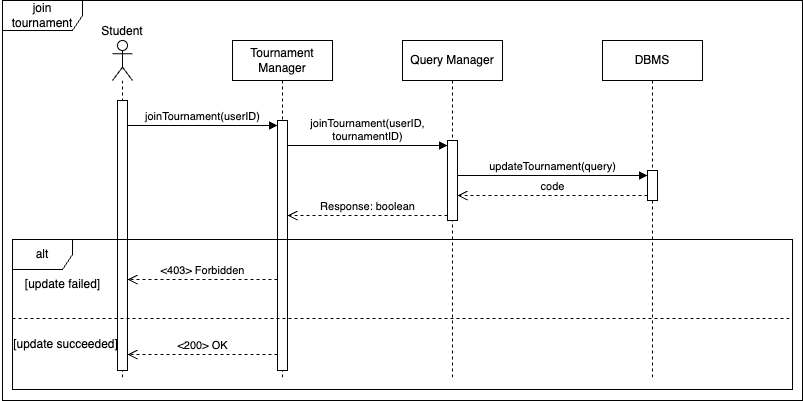
\includegraphics[width=1\linewidth]{src/Join tournament.png}
        \caption{Join tournament}
        \label{fig:Join tournament}
    \end{figure}
    \newpage
    \item \textbf{Create team}\\
    The user navigates to their desired battle thanks to the tournament viewer. If the user is logged in as a student and is not part of any team for that battle, a 'create team' 
    button is displayed that the user can click. This request is handled by the battle manager. If the request is valid, a new team is created for the user. Internal databases are 
    updated accordingly.
    \begin{figure}[h]
        \centering
        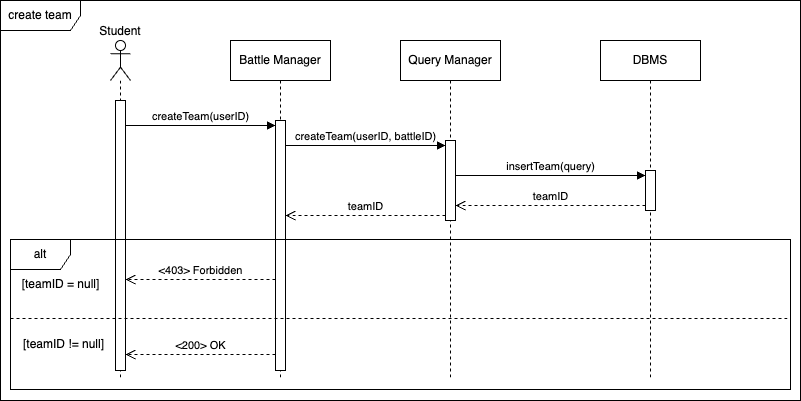
\includegraphics[width=1\linewidth]{src/Create team.png}
        \caption{Create team}
        \label{fig:Create team}
    \end{figure}
    \newpage
    \item \textbf{Join team}\\
    The user navigates to their desired battle thanks to the tournament viewer. If the user is logged in as a student and is not part of any team for that battle, a 'join team by id' 
    button is displayed that the user 
    can click. This request is handled by the battle manager. First the system checks if the id provided is valid for that tournament. If It is not, an error is displayed, otherwise, 
    the user joins that team. Internal databases are updated accordingly.
    \begin{figure}[h]
        \centering
        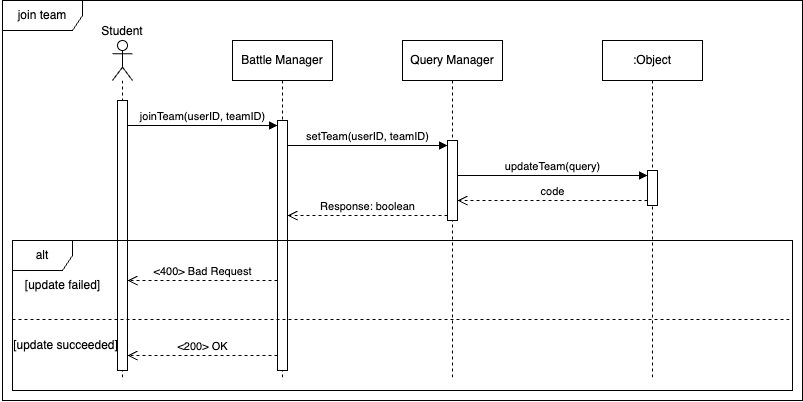
\includegraphics[width=1\linewidth]{src/Join team.png}
        \caption{Join team}
        \label{fig:Join team}
    \end{figure}
    \newpage
    \item \textbf{Join battle}\\
    The user navigates to their desired battle thanks to the tournament viewer. If the user is logged in as a student and is the creator of a team for that battle, a 'join battle' 
    button is displayed that the user can click. 
    This request is handled by the battle manager. First the system checks if the team respects the criteria for that battle. If It does not, an error is displayed, otherwise, 
    the entire team joins that battle. Internal databases are updated accordingly.
    \begin{figure}[h]
        \centering
        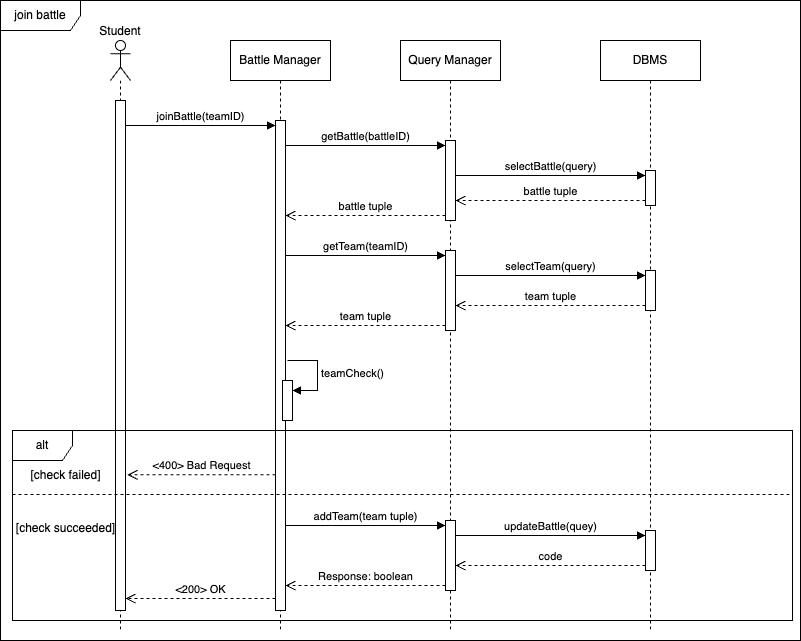
\includegraphics[width=1\linewidth]{src/Join battle.png}
        \caption{Join battle}
        \label{fig:Join battle}
    \end{figure}
    \newpage
    \item \textbf{Submit code}\\
    When a user commits to the main branch of a GitHub repository, GitHub updates its sources. If the user set up a proper automated workflow, the system will be notified by GitHub through the dedicated GitHub API. The system responds updating Its sources, using GitHub API again. After that, the sources are evaluated and the scores are updated. Such update and evaluation is handled by the battle manager.
    \begin{figure} [h]
        \centering
        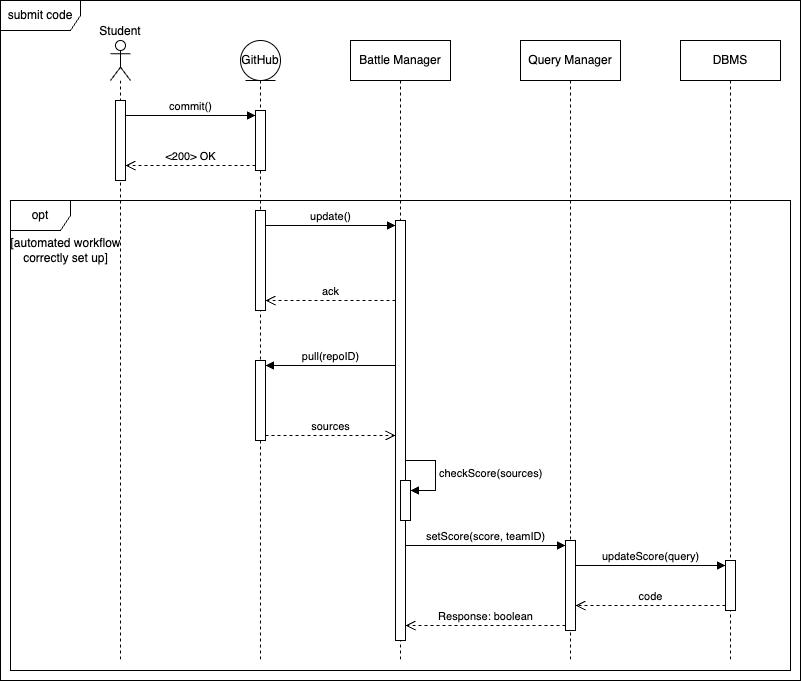
\includegraphics[width=1\linewidth]{src/Submit code.png}
        \caption{Submit code}
        \label{fig:Submit code}
    \end{figure}
    \newpage
    \item \textbf{Create tournament}\\
    If a user is logged in as an educator, a 'create new tournament' button will show up in the main page that the user can click. The whole creation process is handled by the tournament 
    manager. The user chooses their desired settings and submits. The system checks if such settings are applicable (for instance, if the tournament name is not already taken). 
    If they are, the tournament is created, otherwise, an error message will be displayed. Internal databases are updated accordingly.
    \begin{figure}[h]
        \centering
        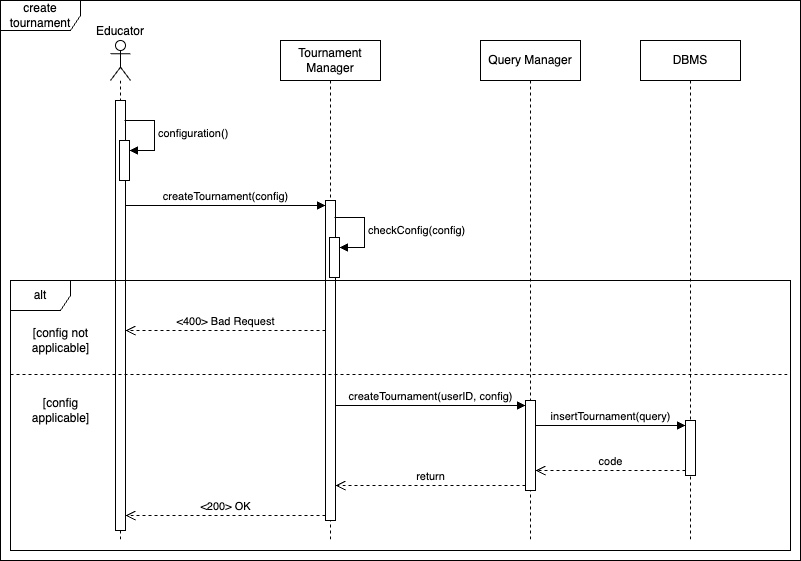
\includegraphics[width=1\linewidth]{src/Create tournament.png}
        \caption{Create tournament}
        \label{fig:Create tournament}
    \end{figure}

    \item \textbf{Edit tournament settings}\\
    The user navigates to their desired tournament thanks to the tournament viewer. If the user is logged in as an educator and is the creator of that tournament, a 'manage tournament' 
    button is displayed that the user can click. After that, the process is similar to the previous one.
    \newpage
    \item \textbf{Create battle}\\
    The user navigates to their desired battle thanks to the tournament viewer. If the user is logged in as an educator and has been granted permission to create battles or is the tournament 
    creator themselves, a 'create new battle' button is displayed that the user can click. The user chooses their desired settings and submits. The system checks if such settings are 
    applicable (for instance, if the battle name for that tournament is not already taken). If they are, the battle is created, otherwise, an error message will be displayed. 
    Internal databases are updated accordingly.
    \begin{figure}[h]
        \centering
        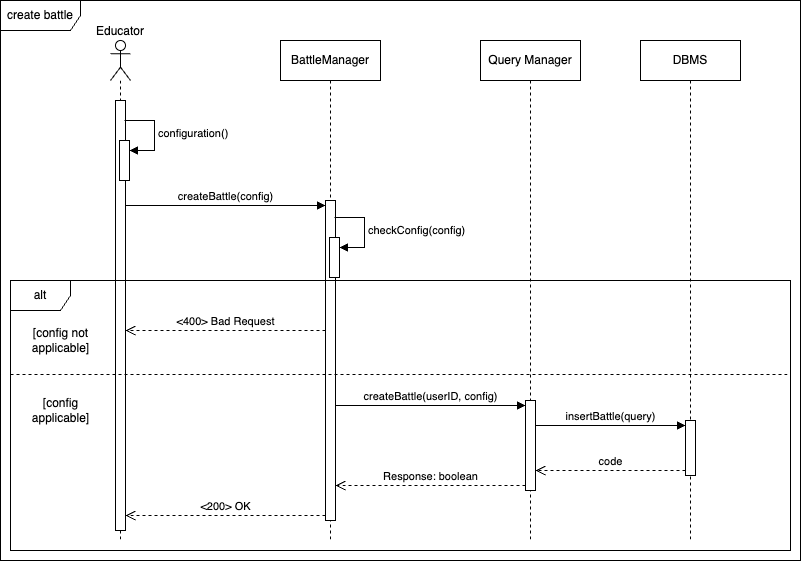
\includegraphics[width=1\linewidth]{src/Create battle.png}
        \caption{Create battle}
        \label{fig:Create battle}
    \end{figure}
    \item \textbf{Edit battle settings}\\
    The user navigates to their desired battle thanks to the tournament viewer. If the user is logged in as an educator and has been granted permission to create battles or is the tournament 
    creator themselves, a 'manage battle' button is displayed that the user can click. After that, the process is similar to the previous one.
    \newpage
    \item \textbf{Review scores}\\
    This process can happen only when a battle is in consolidation phase. The user navigates to their desired battle thanks to the tournament viewer. If the user is logged in as an 
    educator and has been granted permission to create battles or is the tournament creator themselves, a 'review scores' button is displayed that the user can click. 
    The process is handled by the battle manager. Upon submitting, internal databases will be updated accordingly.
    \begin{figure}[h]
        \centering
        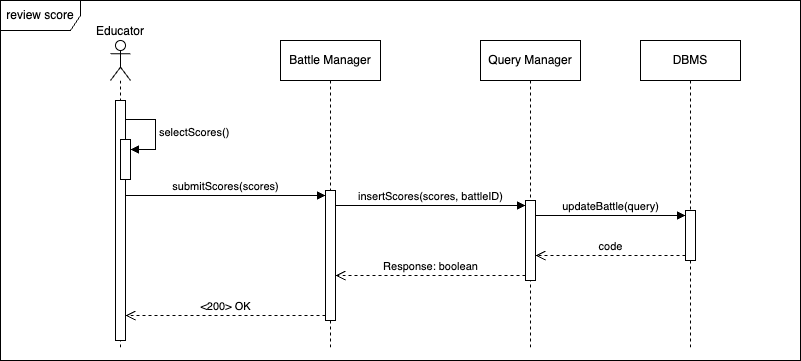
\includegraphics[width=1\linewidth]{src/Review scores.png}
        \caption{Review scores}
        \label{fig:Review scores}
    \end{figure}
    \item \textbf{Close tournament}\\
    This process can only happen when a tournament is ongoing. The user navigates to their desired tournament thanks to the tournament viewer. If the user is logged in as an 
    educator and is the tournament creator, a 'close tournament' button is displayed that the user can click. The process is handled by the tournament manager. Internal databases are updated 
    accordingly.
    \begin{figure}[h]
        \centering
        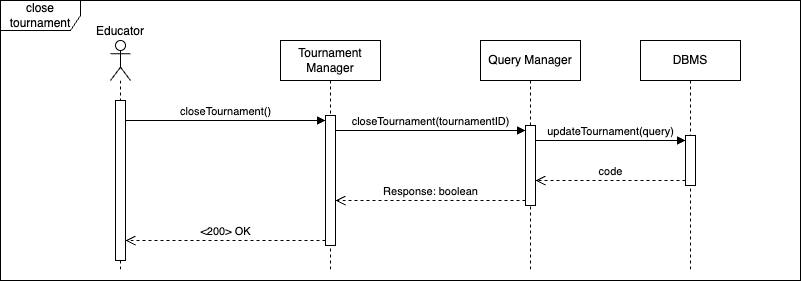
\includegraphics[width=1\linewidth]{src/Close tournament.png}
        \caption{Close tournament}
        \label{fig:Close tournament}
    \end{figure}
    \newpage
    \item \textbf{New tournament notification}\\
    When a new tournament is created in CKB, the tournament manager communicates with the CKB notification service 	in order to send a notification to all users.
    \begin{figure}[h]
        \centering
        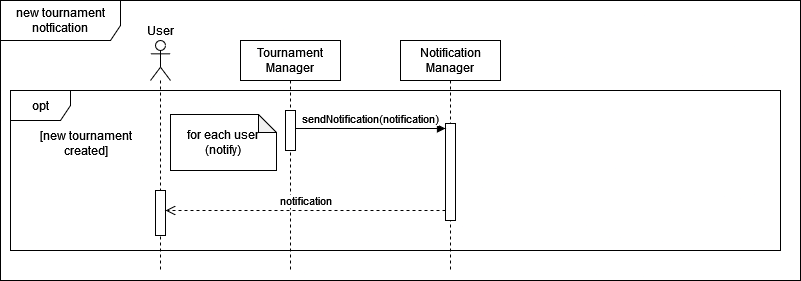
\includegraphics[width=1\linewidth]{src/New tournament notification.png}
        \caption{New tournament notification}
        \label{fig:New tournament notification}
    \end{figure}
    \item \textbf{New battle notification}\\
    When a new battle is created in the scope of a tournament, the battle manager communicates with the CKB notification service in order to send a notification to all users subscribed to that 
    tournament.

    \item \textbf{Battle begins notification}\\
    When a battle begins, the battle manager communicates with GitHub through the dedicated GitHub API in order to create a repository. After that, It communicates with the CKB notification 
    service, which notifies user subscribed to that battle.
    \begin{figure}[h]
        \centering
        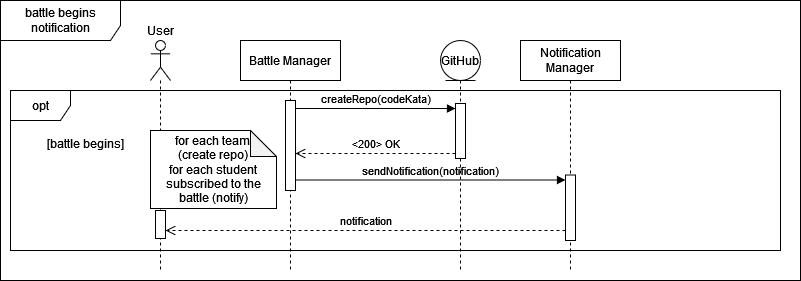
\includegraphics[width=1\linewidth]{src/Battle begins notification.png}
        \caption{Battle begins notification}
        \label{fig:Battle begins notification}
    \end{figure}
    \newpage
    \item \textbf{Badge assignment}\\
    When a tournament closes, the tournament manager communicates with the badge helper, which checks for badges associated with that tournament. If there is any, It will check the 
    requirements for each student. If a user is assigned a badge, the CKB notification service will be called to notify them.
    \begin{figure}[h]
        \centering
        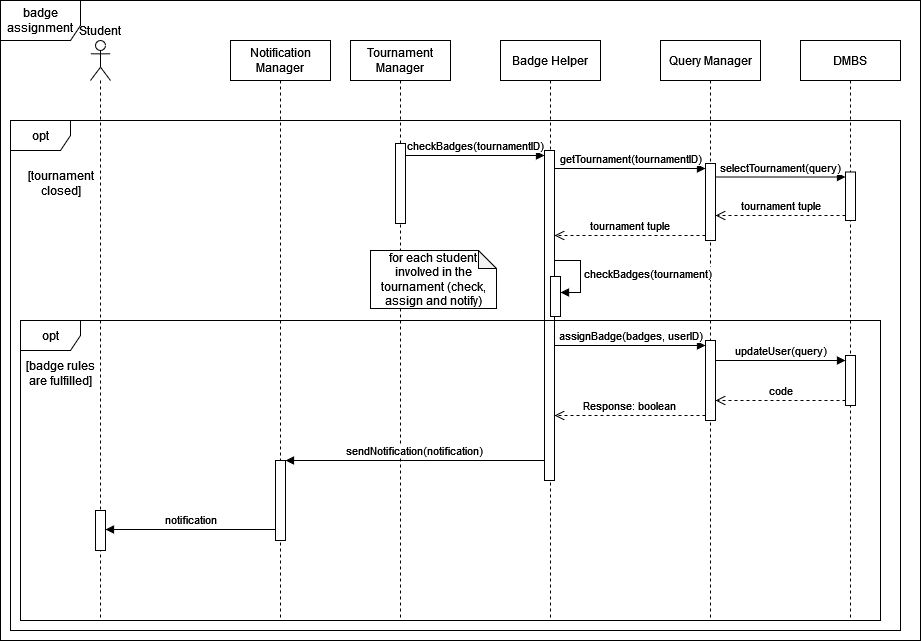
\includegraphics[width=1\linewidth]{src/Badge assignment.png}
        \caption{Badge assignment}
        \label{fig:Badge assignment}
    \end{figure}
\end{itemize}

\newpage
\subsection{Component Interfaces}
This section lists all the methods offered by each component interface to the other components.
\begin{figure}[h]
    \centering
    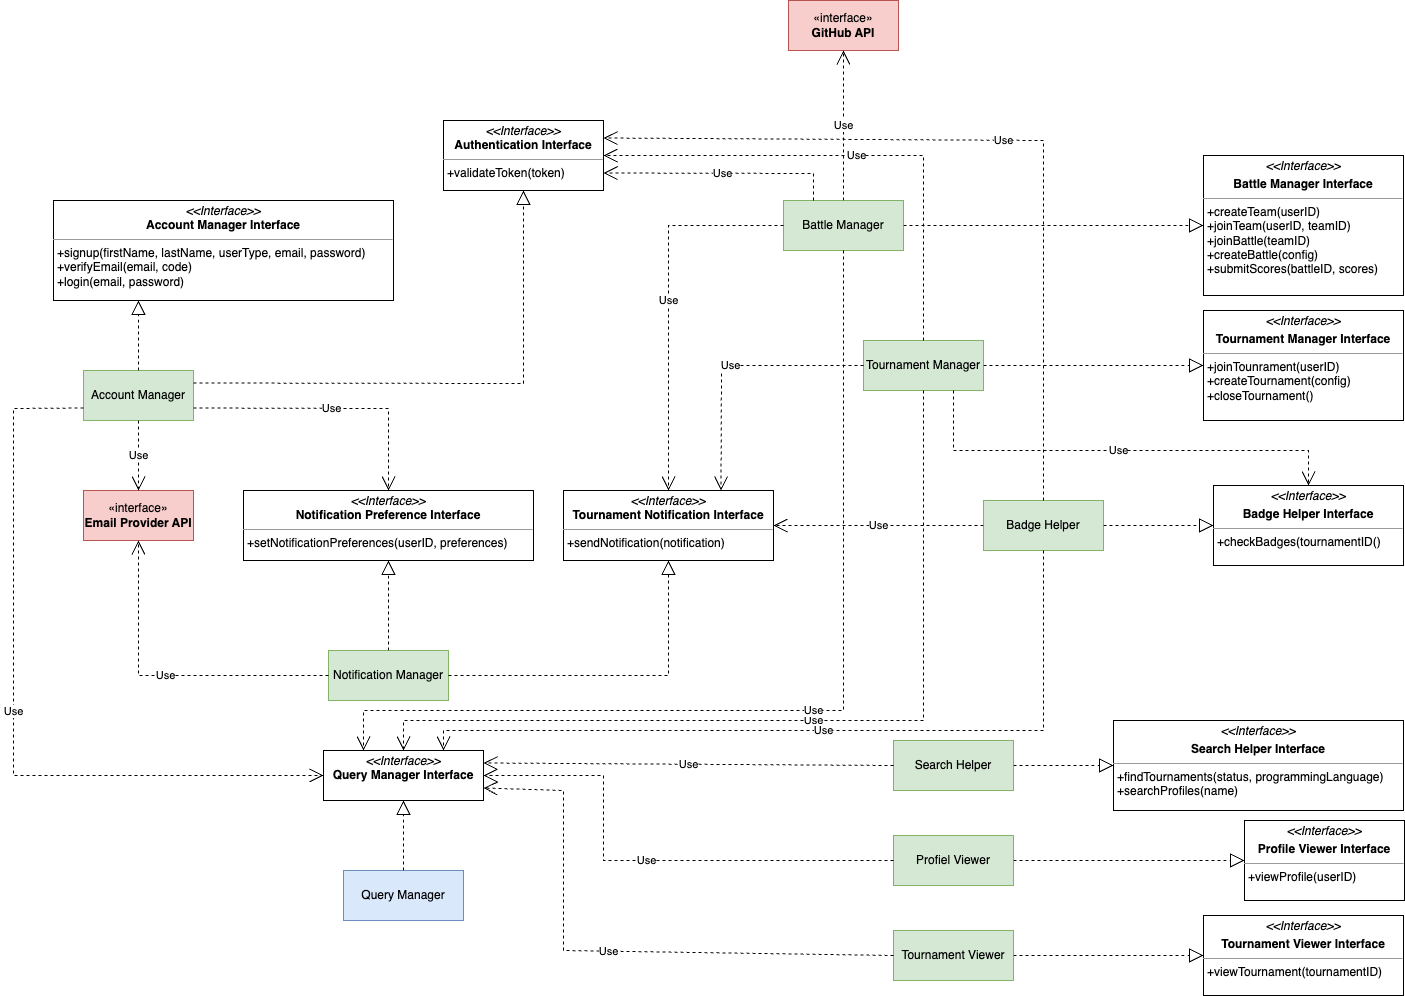
\includegraphics[width=1\linewidth]{src/Class Diagram with interfaces of the CKB System.png}
    \caption{Class Diagram with interfaces of the CKB System}
    \label{fig:Class Diagram with interfaces of the CKB System}
\end{figure}
\subsection{Selected architectural styles and patterns}
\begin{itemize}
    \item \textbf{Three layer four tier}\\
    This architecture offers several benefits. It allows the distinction of layers (presentation, logic, data) and tiers (client, web server, application server, DBMS), which makes the system more modular and easier to maintain. Such separation also allows better scalability and better workload distribution across multiple servers. Finally, load balancing and caching techniques are available to further increase performance and availability.

    \item \textbf{RESTful APIs}\\
    The API is based on standard web technologies, like JSON or XML, allowing better integration with other systems. It is stateless, which makes the development easier. It also promotes simplicity and scalability.\\
    \item \textbf{Adapter pattern}\\
    The Adapter Pattern seamlessly integrates different components, standardizing interfaces and ensuring flexibility. It hides the underlying complexity and provides a set of high-level functions. 
\end{itemize}

\vspace{1cm}
    
\subsection{Other design decisions}
\begin{itemize}
    \item SQL database
    SQL databases offer high scalability and decent performance for structured data. It follows ACID principles and ensures data integrity. Overall, It is a good compromise for performance, consistency, reliability and ease of use.
\end{itemize}